% Editable revision of the user-supplied ThreatLens (1).pdf.
% Compile with pdfLaTeX twice. No external images or bibliography files needed.
% The numerical results are retained from the supplied draft, not re-measured.
\documentclass[conference,letterpaper]{IEEEtran}
\usepackage[T1]{fontenc}
\usepackage[utf8]{inputenc}
\usepackage{mathptmx}
\usepackage{amsmath}
\usepackage{booktabs,array,tabularx}
\usepackage{tikz}
\usetikzlibrary{arrows.meta,positioning}
\usepackage[hidelinks]{hyperref}
\urlstyle{same}
\hypersetup{
  pdftitle={ThreatLens: An LLM-Agentic Multi-Scanner Architecture for Automated Compliance Mapping and Threat Modeling},
  pdfauthor={Jignesh Sonewane; Soham Pashine; Bhargav Bawane; Professor Pankaj Sonewane},
  pdfsubject={Multi-scanner security review and retrieval-grounded compliance mapping},
  pdfkeywords={ThreatLens, security review, compliance mapping, vulnerability detection, RAG}
}
\newcolumntype{Y}{>{\raggedright\arraybackslash}X}
\newcommand{\authorentry}[3]{%
  \begin{minipage}[t]{0.47\textwidth}\centering
  {\normalsize #1\par}\vspace{3pt}
  {\small #2\par
  G. H. Raisoni College of Engineering\par
  Nagpur, India\par}
  {\footnotesize\href{mailto:#3}{#3}\par}
  \end{minipage}}
\setlength{\emergencystretch}{1.3em}
\renewcommand{\arraystretch}{1.12}

\title{ThreatLens: An LLM-Agentic Multi-Scanner Architecture\\
for Automated Compliance Mapping and Threat Modeling}
\author{%
  \authorentry{Jignesh Sonewane}{Department of Computer Science and Engineering}{jignesh.sonewane.cyb@ghrce.raisoni.net}\hspace{0.02\textwidth}%
  \authorentry{Soham Pashine}{Department of Computer Science and Engineering}{soham.pashine.cyb@ghrce.raisoni.net}\\[12pt]
  \authorentry{Bhargav Bawane}{Department of Computer Science and Engineering}{bhargav.bawane.cyb@ghrce.raisoni.net}\hspace{0.02\textwidth}%
  \authorentry{Professor Pankaj Sonewane}{DIC Department}{pankaj.sonewane@raisoni.net}%
}

\begin{document}
\maketitle

\begin{abstract}
Security tools can identify suspicious code, exposed credentials and vulnerable dependencies, but their findings still need to be checked, prioritised and related to organisational requirements. ThreatLens brings these tasks into one review workflow. The prototype combines Semgrep, Bandit, TruffleHog, dependency auditing, log-anomaly analysis and a large-language-model code reviewer through an asynchronous task pipeline. It normalises overlapping findings and retrieves candidate control clauses from a 534-entry knowledge base covering five compliance frameworks. The resulting reports place source evidence, proposed control mappings, severity and remediation guidance together for human review. A preliminary evaluation reports 34 detections among 37 seeded defects in a 47-file Flask application, a mean retrieval precision of 0.868 at rank ten, and an end-to-end time of 80.7 seconds. These figures describe a limited benchmark, not field validation; the phase timings and evaluation records require further reconciliation. The contribution is an integrated approach to evidence-based security review, rather than a replacement for an analyst or a guarantee of compliance.
\end{abstract}

\begin{IEEEkeywords}
static analysis, vulnerability detection, compliance mapping, retrieval-augmented generation, threat modeling, DevSecOps.
\end{IEEEkeywords}

\section{Introduction}
Finding a security issue is only the beginning of a review. A developer must understand the affected code, decide whether the issue is reachable in practice, and identify a change that preserves the application's behaviour. An auditor may also need to understand which control the evidence relates to. When scanners, control catalogues and reports are kept separately, much of this work becomes manual.

Two problems motivate ThreatLens. First, different tools describe the same issue in different ways, making duplicate findings and inconsistent priorities difficult to manage. Second, a code-level observation does not translate directly into a compliance conclusion. A suspected injection flaw, for example, may be relevant to several controls, but its presence alone does not establish an organisation-wide compliance failure.

ThreatLens connects detection, evidence review, candidate control mapping and reporting. Its contribution is threefold: a common finding format for complementary scanners; retrieval-grounded mapping that keeps the supporting control text available; and workspace-scoped delivery of findings and reports. The system supports threat analysis by organising evidence. It does not establish an exploit path merely by displaying a relationship between findings.

This paper describes the six-engine prototype configuration and its preliminary evaluation. Later deployments may differ in their components and behaviour. The reported measurements therefore apply only to the configuration and fixture described here.

\section{Related Work}
Zhou et al. review the use of large language models for vulnerability detection and repair~\cite{zhou}. Their survey provides a basis for considering language-model review alongside established analysis tools, rather than treating it as a substitute for them. Shestov et al. investigate fine-tuning for vulnerability detection~\cite{shestov}. That work does not, by itself, validate the confidence threshold used in this prototype.

Uddin et al. organise deep-learning-based vulnerability detection around dataset construction, representation, modelling and evaluation~\cite{uddin}. These distinctions matter when comparing tools: a result on a seeded application cannot establish performance across languages, repositories or deployment environments.

Lewis et al. introduce retrieval-augmented generation, combining generation with access to retrieved material~\cite{lewis}. ThreatLens uses this general idea to supply control clauses as context. Sentence-BERT demonstrates how sentence embeddings can support semantic similarity search~\cite{sbert}. Retrieval can make evidence easier to inspect, but a relevant passage does not guarantee a correct compliance interpretation.

SecretBench provides a labelled dataset for studying software-secret detection~\cite{secretbench}. It illustrates the importance of evaluating genuine secrets separately from look-alike strings. ThreatLens similarly requires contextual review of secret alerts. CVSS~3.1 supplies the scoring vocabulary used in the prototype~\cite{cvss}; a generated score and vector still need to agree with the evidence and the metric definitions.

\section{System Architecture}
The workflow in Fig.~\ref{fig:architecture} separates ingestion, analysis, interpretation and delivery. FastAPI accepts requests, while Celery workers perform long-running work through a Redis broker. Keeping that work outside the request handler allows the interface to report progress without holding an HTTP request open for the entire scan.

\begin{figure}[t]
\centering
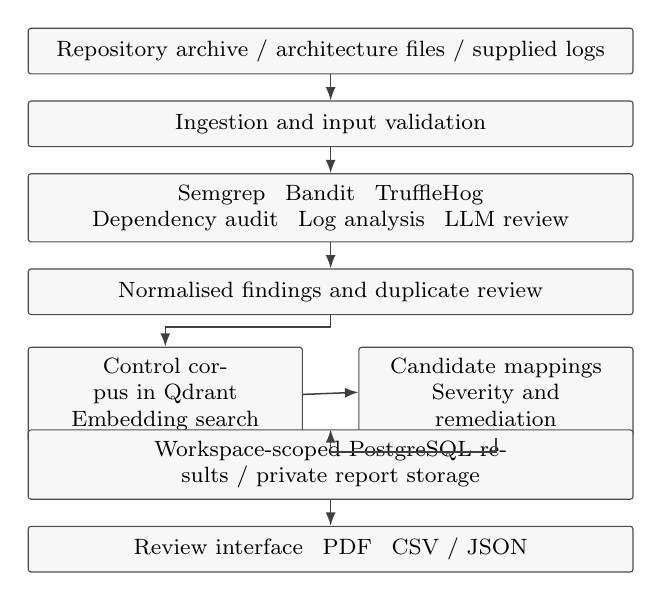
\begin{tikzpicture}[
  font=\footnotesize,
  stage/.style={draw=black!70,rounded corners=1pt,fill=black!3,
    align=center,text width=7.4cm,minimum height=0.58cm,inner sep=4pt},
  side/.style={stage,text width=3.2cm,minimum height=0.72cm},
  flow/.style={-{Latex[length=1.7mm]},draw=black!75,line width=0.55pt},
  node distance=0.33cm]
  \node[stage] (input) {Repository archive / architecture files / supplied logs};
  \node[stage,below=of input] (ingest) {Ingestion and input validation};
  \node[stage,below=of ingest] (scan) {Semgrep \enspace Bandit \enspace TruffleHog\\
    Dependency audit \enspace Log analysis \enspace LLM review};
  \node[stage,below=of scan] (merge) {Normalised findings and duplicate review};
  \node[side,below=0.4cm of merge.south west,anchor=north west] (rag)
    {Control corpus in Qdrant\\Embedding search};
  \node[side,below=0.4cm of merge.south east,anchor=north east] (map)
    {Candidate mappings\\Severity and remediation};
  \node[stage,below=1.45cm of merge] (store) {Workspace-scoped PostgreSQL results / private report storage};
  \node[stage,below=of store] (out) {Review interface \enspace PDF \enspace CSV / JSON};
  \draw[flow] (input)--(ingest);
  \draw[flow] (ingest)--(scan);
  \draw[flow] (scan)--(merge);
  \draw[flow] (merge.south) -- ++(0,-0.15) -| (rag.north);
  \draw[flow] (rag.east)--(map.west);
  \draw[flow] (map.south) -- ++(0,-0.18) -| (store.north);
  \draw[flow] (store)--(out);
\end{tikzpicture}
\caption{Prototype review workflow. Retrieved controls support interpretation; saved findings and reports remain separate from the control index. Progress is reported during processing.}
\label{fig:architecture}
\end{figure}

The prototype's reported technology choices are summarised in Table~\ref{tab:stack}. These are configuration details for the study, not recommendations to install the listed versions in a new production system. Tool versions, rulesets, model identifiers and the control corpus should be recorded together when reproducing a run.

\begin{table}[t]
\caption{Technology Configuration Reported for the Prototype}
\label{tab:stack}
\centering\footnotesize
\begin{tabularx}{\columnwidth}{@{}lY@{}}
\toprule
Layer & Technology \\
\midrule
API / workers & Python 3.11, FastAPI 0.110, Celery 5.x, Redis 7 \\
Model / retrieval & Groq-hosted Llama-3-70B, LangChain 0.2, all-MiniLM-L6-v2, Qdrant \\
Data / access & PostgreSQL 15, Supabase Auth and Storage \\
Reporting & WeasyPrint 60, Jinja2 3, matplotlib 3.9 \\
Frontend & React 18, TypeScript, TanStack Start / Query \\
\bottomrule
\end{tabularx}
\end{table}

\section{Scanners and Compliance Knowledge Base}
\subsection{Complementary Analysis}
Scanner outputs are converted into records containing severity, a weakness identifier where available, and source-file and line information. The prototype groups overlaps using path, line and CWE, retaining the highest reported severity. This is a practical duplicate heuristic, not a proof that two reports describe the same underlying flaw. Distinct findings can share a location, and line numbers can change between revisions.

Semgrep supplies pattern-based checks for common web and language-specific weaknesses. Bandit adds Python syntax-tree checks, including potentially unsafe subprocess use and weak cryptographic constructs. TruffleHog examines suspected credentials. Dependency auditing uses pip-audit and npm audit to identify known vulnerable package versions and available fixes. Tool severity labels are normalised for presentation; they do not replace an assessment of reachability and impact.

Log analysis combines rules with an Isolation Forest. The reported rule configuration includes repeated authentication failures, injection-like strings and unusual HTTP methods. The anomaly model uses request rate, error rate and endpoint diversity, with contamination set to 0.05. An anomaly is a reason to investigate, not evidence that an attack succeeded.

The language-model reviewer examines up to 30 files, with an 8~KB limit per file, and returns structured JSON. The prototype discards responses with a reported confidence below 0.70. This value is a filtering heuristic, not a calibrated probability. File selection and truncation therefore belong in the coverage statement: a completed scan does not mean that every file received model review.

\subsection{Retrieval-Grounded Control Mapping}
The reported corpus contains 534 entries: 89 labelled GDPR, 67 SOC~2, 114 ISO~27001, 156 PCI~DSS and 108 NIST~CSF. These counts describe the prototype's selected material, not authoritative totals for current framework editions. The original corpus labels are insufficient to establish that every entry belongs to the claimed edition; version and source reconciliation remain necessary.

Each entry carries a framework label, control identifier, title and text. The all-MiniLM-L6-v2 model produces 384-dimensional, normalised embeddings, which are stored in Qdrant and compared using cosine similarity. For each finding, retrieval returns up to 12 candidate clauses, optionally restricted by framework. The mapper then uses those passages to propose a relationship between the evidence and a control.

A useful mapping must expose both sides of that relationship: what the scanner observed and what the cited requirement actually says. Schema validation checks the response structure, but cannot establish that the interpretation is correct. Human review remains necessary, especially for organisational obligations that cannot be established from source code alone.

\section{Task Pipeline and Security Boundaries}
The interpretation stage first retrieves candidate clauses, then produces structured mappings. Severity assessment and remediation planning follow, after which findings are saved and summarised for reporting. The prototype groups suggested actions into immediate, short-term and longer-term work. Those labels help prioritisation; they are not contractual remediation deadlines.

The reported orchestration uses bounded retries with exponential backoff for provider failures. It isolates scanner failures so that one unavailable engine does not discard findings from the others. This design needs an explicit coverage record: returning no findings after an engine fails must not be presented as a clean result. Failed, skipped and truncated checks should remain visible alongside completed checks.

Supplied code and logs are untrusted data. Prompt delimiters help distinguish that data from instructions, but do not eliminate prompt injection. Likewise, structured output does not establish the truth of a generated explanation. Proposed fixes require inspection and testing before use.

The prototype describes workspace-membership checks, JWT verification, PostgreSQL row-level security and private report storage. Downloads use short-lived signed links after authorisation. Progress is delivered through an authenticated WebSocket, with polling as a fallback. CSV output requires spreadsheet-formula protection in addition to normal quoting. These controls address different risks and must be tested independently; their presence is not proof of complete tenant isolation.

The reported upload safeguards include path-traversal rejection, a 1,000-file cap, a 100-fold expansion limit and task timeouts. Non-root workers and JSON serialisation reduce exposure, but do not make uploaded content safe. Dependency inspection must avoid executing untrusted package installation steps, and report generation must restrict resource access. These are deployment requirements, not guarantees established by the benchmark.

\section{Preliminary Evaluation and Discussion}
\subsection{Experimental Scope}
The preliminary evaluation uses a 47-file Flask application with 37 seeded defects and containerised PostgreSQL, Redis and Qdrant. The reported host had 32~GB of RAM and an NVIDIA RTX~4060; the language-model service was remote, so the local GPU is not evidence of local inference performance. Tables~\ref{tab:detection}--\ref{tab:timing} reproduce the available measurements. Raw run logs were not available for independent validation.

\begin{table}[t]
\caption{Reported Detection Results on the Seeded Benchmark}
\label{tab:detection}
\centering\footnotesize
\begin{tabularx}{\columnwidth}{@{}Yrrr@{}}
\toprule
Scanner & Seeded & Found & Recall \\
\midrule
Semgrep & 12 & 11 & 91.7\% \\
Bandit & 8 & 8 & 100.0\% \\
TruffleHog & 3 & 3 & 100.0\% \\
Dependency audit & 3 & 3 & 100.0\% \\
Log analysis & 5 & 4 & 80.0\% \\
LLM review & 6 & 5 & 83.3\% \\
\midrule
Total reported & 37 & 34 & 91.9\% \\
\bottomrule
\end{tabularx}
\end{table}

\subsection{Detection and Coverage}
The reported aggregate recall is $34/37=91.9\%$. Bandit, TruffleHog and dependency auditing found all seeded items assigned to them in this small fixture. Such results should not be interpreted as perfect detection outside the fixture.

The evaluation record also describes six cross-engine overlaps, but lacks enough item-level detail to reconcile those overlaps with the table's denominator. The recorded explanation attributes misses to truncation and confidence filtering, yet lists two explanations against one missed LLM item. The archived ground-truth list and per-engine outputs are therefore needed before drawing conclusions about unique-defect recall or the exact cause of a miss.

An approximately 16\% false-positive measure is also recorded without a denominator or adjudication procedure. It is not treated here as a verified false-positive rate. A repeatable evaluation should report true positives, false positives and false negatives separately, together with the rules used to label ambiguous findings.

\begin{table}[t]
\caption{Reported Retrieval Results by Corpus Label}
\label{tab:retrieval}
\centering\footnotesize
\begin{tabularx}{\columnwidth}{@{}Yrrr@{}}
\toprule
Framework label & P@5 & P@10 & First-hit rank \\
\midrule
GDPR & 0.91 & 0.88 & 1.4 \\
SOC 2 & 0.89 & 0.86 & 1.6 \\
ISO 27001 & 0.93 & 0.89 & 1.2 \\
PCI DSS & 0.88 & 0.84 & 1.7 \\
NIST CSF & 0.90 & 0.87 & 1.5 \\
\midrule
Mean & 0.902 & 0.868 & 1.48 \\
\bottomrule
\end{tabularx}
\end{table}

\subsection{Retrieval Quality}
Table~\ref{tab:retrieval} reports a mean P@10 of 0.868 and a mean first relevant result at rank 1.48. Precision at $k$ measures the fraction of the first $k$ retrieved entries judged relevant. The record does not include the query set, relevance labels or agreement between reviewers. These figures are consequently preliminary. They assess reported retrieval relevance, not the accuracy of every generated mapping or an organisation's compliance status.

\begin{table}[t]
\caption{Reported Timing for the 47-File Benchmark}
\label{tab:timing}
\centering\footnotesize
\begin{tabularx}{\columnwidth}{@{}Yr@{}}
\toprule
Phase & Time (s) \\
\midrule
Ingestion & 1.2 \\
Semgrep / Bandit / TruffleHog & 26.1 \\
Dependency audit & 6.2 \\
LLM review (30 files) & 28.4 \\
Compliance mapping (34 findings) & 17.6 \\
Report generation & 0.9 \\
\midrule
Sum of listed phases & 80.4 \\
Reported end-to-end time & 80.7 \\
\bottomrule
\end{tabularx}
\vspace{3pt}
\parbox{\columnwidth}{\footnotesize The 0.3-second difference is not explained by the supplied record. It is not assigned to a particular phase or assumed overhead.}
\end{table}

\subsection{Runtime and Reproducibility}
The listed phases add to 80.4 seconds, whereas the reported end-to-end time is 80.7 seconds. Table~\ref{tab:timing} makes that difference explicit. Model review and mapping account for 46.0 seconds, roughly 57\% of the reported total. Without provider traces and repeated measurements, this does not isolate network latency from other processing costs. Nor does the single run establish throughput under concurrent load.

The prototype record lists 89 passing tests and four skipped tests. These historical counts do not establish the status of a later build. A reproducibility package should include the seeded application, labelled defects, rulesets, model and prompt versions, corpus snapshot, test commands and raw timing logs. Evaluation on additional repositories is needed to examine language coverage, false positives and sensitivity to project size.

\section{Conclusion and Future Work}
ThreatLens provides a way to review scanner findings, their supporting evidence and candidate compliance mappings in one workflow. Its value lies in connecting these steps while keeping the reviewer in control. The prototype's reported results are encouraging, but the small seeded fixture and incomplete evaluation records limit the conclusions that can be drawn.

The next research priority is a reproducible benchmark with reconciled ground truth, a documented relevance-labelling procedure, versioned control sources and repeated timing measurements.

% Manual final-page column break; revisit if the paper content is changed.
\newpage
Further work can examine data-flow analysis, broader language coverage and carefully reviewed remediation proposals. Any later repository or CI integration should retain an explicit approval boundary before publishing changes. A scan with no findings is not proof that a system is secure, and an automated control mapping is not certification.

\section*{Acknowledgment}
The authors thank the faculty of the Department of Computer Science and Engineering and the DIC Department at G.~H.~Raisoni College of Engineering, Nagpur, for their guidance. They also acknowledge the maintainers of the open-source tools used in the prototype.

\begin{thebibliography}{7}
\bibitem{zhou}
X. Zhou, S. Cao, X. Sun, and D. Lo, ``Large language model for vulnerability detection and repair: Literature review and the road ahead,'' arXiv:2404.02525, 2024. [Online]. Available: \url{https://arxiv.org/abs/2404.02525}

\bibitem{shestov}
A. Shestov, R. Levichev, R. Mussabayev, E. Maslov, A. Cheshkov, and P. Zadorozhny, ``Finetuning large language models for vulnerability detection,'' arXiv:2401.17010, 2024. [Online]. Available: \url{https://arxiv.org/abs/2401.17010}

\bibitem{uddin}
M. N. Uddin, Y. Zhang, and X. Hei, ``Deep learning aided software vulnerability detection: A survey,'' arXiv:2503.04002, 2025. [Online]. Available: \url{https://arxiv.org/abs/2503.04002}

\bibitem{lewis}
P. Lewis et al., ``Retrieval-augmented generation for knowledge-intensive NLP tasks,'' in \emph{Advances in Neural Information Processing Systems}, vol. 33, 2020, pp. 9459--9474. [Online]. Available: \url{https://arxiv.org/abs/2005.11401}

\bibitem{sbert}
N. Reimers and I. Gurevych, ``Sentence-BERT: Sentence embeddings using siamese BERT-networks,'' in \emph{Proc. EMNLP-IJCNLP}, 2019. [Online]. Available: \url{https://arxiv.org/abs/1908.10084}

\bibitem{secretbench}
S. K. Basak, L. Neil, B. Reaves, and L. Williams, ``SecretBench: A dataset of software secrets,'' in \emph{Proc. IEEE/ACM MSR}, 2023. [Online]. Available: \url{https://arxiv.org/abs/2303.06729}

\bibitem{cvss}
FIRST.Org, Inc., ``Common Vulnerability Scoring System v3.1: Specification document,'' 2019. [Online]. Available: \url{https://www.first.org/cvss/v3-1/specification-document}
\end{thebibliography}
\end{document}
